\documentclass[12pt,a4paper]{article}
\usepackage[utf8]{inputenc}
\usepackage[T1]{fontenc}
\usepackage{amsmath, amssymb, amsfonts}
\usepackage{graphicx}
\usepackage{float}
\usepackage{geometry}
\usepackage{xcolor}
\geometry{margin=2.5cm}

\title{Hitra Fourierova transformacija}
\author{Filip Jesenšek (28231064)}
\date{\today}

\begin{document}

\maketitle

\begin{abstract}
V poročilu obravnavamo uporabo hitre Fourierove transformacije (FFT) za izračun avtokorelacijske funkcije in spektrogramov signalov. S FFT izračunamo avtokorelacijo in spektrograme dveh referenčnih signalov sove (bubomono in bubo2mono) ter štirih mešanih signalov (mix, mix1, mix2, mix22). Z metodo normalizirane avtokorelacije in iskanjem dominantnih period identificiramo, katera sova nastopa v najbolj zašumljenih signalih (mix2 in mix22). Rezultate vizualiziramo s časovnimi poteki, avtokorelacijskimi funkcijami in spektrogrami (waterfall diagrami), ki prikazujejo frekvenčno vsebino signala skozi čas. Ugotovimo, da je v obeh zašumljenih signalih prisotna sova \textit{bubomono}.
\end{abstract}

\section{Uvod}

Hitra Fourierova transformacija (FFT) je temeljno orodje za analizo signalov, ki omogoča hiter prehod iz časovne v frekvenčno domeno s časovno zahtevnostjo $\mathcal{O}(N \log N)$. V nalogi želimo s pomočjo FFT izračunati avtokorelacijsko funkcijo signalov in njihove spektrograme ter identificirati oglašanje sove v šumnih okoljih.

Avtokorelacija je definirana kot:
\begin{equation}
C(g,h)_n = \frac{1}{N} \sum_{k=0}^{N-1} g_{k+n} h_k.
\end{equation}

Pri uporabi FFT avtokorelacijo računamo kot:
\begin{equation}
C(h,h)_n = \mathcal{F}^{-1}\big[|\mathcal{F}h|^2\big],
\end{equation}
kjer uporabimo nepristransko oceno:
\begin{equation}
C(h,h)_n^{\text{unbiased}} = \frac{1}{N-n} \sum_{k=0}^{N-n-1} h_{k+n} h_k.
\end{equation}

Normalizirana avtokorelacija je podana z:
\begin{equation}
\tilde{C}(h,h)_n = \frac{C(h,h)_n - \langle h \rangle^2}{C(h,h)_0 - \langle h \rangle^2},
\end{equation}
kjer je $\langle h \rangle$ povprečje signala:
\begin{equation}
\langle h \rangle = \frac{1}{N} \sum_{k=0}^{N-1} h_k.
\end{equation}

Spektrogram (waterfall diagram) je vizualizacija spektra signala skozi čas, kjer je na x-osi čas, na y-osi frekvenca, barva pa predstavlja amplitudo (magnitudo) frekvenčne komponente v decibelih.

\section{Metodologija}

\subsection{Računanje avtokorelacije z FFT}
Signale dolžine $N$ smo najprej podvojili z ničlami (zero-padding) na dolžino $2N$, da smo preprečili cirkularno konvolucijo. Nato smo izračunali FFT, kvadrirali magnitudo in izvedli inverzno FFT. Dobljeni avtokorelaciji smo dodali deljenje z $N-n$ za nepristransko oceno.

\subsection{Računanje spektrogramov}
Spektrograme smo izračunali s pomočjo funkcije \texttt{spectrogram} iz knjižnice \texttt{scipy.signal}. Uporabili smo naslednje parametre:
\begin{itemize}
    \item Dolžina okna: 2048 vzorcev (približno 46 ms pri vzorčni frekvenci 44.1 kHz)
    \item Prekrivanje oken: 50\%
    \item Frekvenčno območje: 0-5000 Hz (zadostuje za frekvenčno območje sove)
    \item Barvna lestvica: \textit{viridis}
    \item Enote magnitude: decibeli (dB)
\end{itemize}

\subsection{Iskanje dominantnih period}
V normalizirani avtokorelaciji smo poiskali vrhove nad pragom 0.15 ter jih pretvorili v periode in frekvence. Podobnost med testnim signalom in referencama smo ocenili s primerjavo treh najmočnejših period.

\section{Rezultati in analiza}

\subsection{Analiza signalov sove}

Na voljo so bili signali:
\begin{itemize}
    \item \texttt{bubomono} in \texttt{bubo2mono} (referenčna signala sove),
    \item \texttt{mix}, \texttt{mix1}, \texttt{mix2}, \texttt{mix22} (mešani signali z različnimi stopnjami šuma).
\end{itemize}
Frekvenco vzorčenja smo ocenili na 44.1 kHz, kar je standardna frekvenca za avdio posnetke. Skupna dolžina posnetkov je približno 2-3 sekunde.

\subsection{Spektrogrami referenčnih signalov}

Slika \ref{fig:bubomono_spectrogram} prikazuje spektrogram referenčnega signala \texttt{bubomono}. Opazimo lahko značilne frekvenčne pasove pri osnovni frekvenci približno 379 Hz in njenih harmonikih. Barva prikazuje moč signala v decibelih – temnejša/rdečkasta področja predstavljajo višjo amplitudo.

\begin{figure}[H]
    \centering
    \includegraphics[width=0.9\textwidth]{bubomono_spectrogram.pdf}
    \caption{Spektrogram referenčnega signala \texttt{bubomono}. Opazni so značilni frekvenčni vrhovi pri 379 Hz in višjih harmonikih.}
    \label{fig:bubomono_spectrogram}
\end{figure}

Slika \ref{fig:bubo2mono_spectrogram} prikazuje spektrogram referenčnega signala \texttt{bubo2mono}. Njegova osnovna frekvenca je nekoliko nižja, približno 350 Hz, kar je razvidno iz premika frekvenčnih pasov proti nižjim frekvencam.

\begin{figure}[H]
    \centering
    \includegraphics[width=0.9\textwidth]{bubo2mono_spectrogram.pdf}
    \caption{Spektrogram referenčnega signala \texttt{bubo2mono} z osnovno frekvenco pri 350 Hz.}
    \label{fig:bubo2mono_spectrogram}
\end{figure}

\subsection{Spektrogrami mešanih signalov}

Sliki \ref{fig:mix2_spectrogram} in \ref{fig:mix22_spectrogram} prikazujeta spektrograma najbolj zašumljenih signalov \texttt{mix2} in \texttt{mix22}. Kljub močnemu ozadju lahko še vedno opazimo frekvenčne vrhove pri 379 Hz, kar ustreza osnovni frekvenci sove \texttt{bubomono}.

\begin{figure}[H]
    \centering
    \includegraphics[width=0.9\textwidth]{mix2_spectrogram.pdf}
    \caption{Spektrogram signala \texttt{mix2}. Kljub šumu so še vedno vidni vrhovi pri 379 Hz.}
    \label{fig:mix2_spectrogram}
\end{figure}

\begin{figure}[H]
    \centering
    \includegraphics[width=0.9\textwidth]{mix22_spectrogram.pdf}
    \caption{Spektrogram signala \texttt{mix22}. Frekvenčni vzorec se ujema z referenco \texttt{bubomono} (379 Hz).}
    \label{fig:mix22_spectrogram}
\end{figure}

\subsection{Primerjava spektrogramov}

Za lažjo vizualno primerjavo smo na sliki \ref{fig:mix22_spectrograms_comparison} prikazali spektrograme referenčnih signalov in testnega signala \texttt{mix22} skupaj. Iz primerjave je jasno razvidno, da se frekvenčni vzorec testnega signala najbolj ujema s signalom \texttt{bubomono} – oba imata osnovno frekvenco pri 379 Hz.

\begin{figure}[H]
    \centering
    \includegraphics[width=0.9\textwidth]{mix22_spectrograms_comparison.pdf}
    \caption{Primerjava spektrogramov: \texttt{bubomono} (zgoraj), \texttt{bubo2mono} (sredina) in \texttt{mix22} (spodaj). Testni signal se po frekvenčni vsebini najbolj ujema z \texttt{bubomono}.}
    \label{fig:mix22_spectrograms_comparison}
\end{figure}

Podobno slika \ref{fig:mix2_spectrograms_comparison} prikazuje primerjavo za signal \texttt{mix2}.

\begin{figure}[H]
    \centering
    \includegraphics[width=0.9\textwidth]{mix2_spectrograms_comparison.pdf}
    \caption{Primerjava spektrogramov za \texttt{mix2}. Prav tako opazimo ujemanje z referenco \texttt{bubomono}.}
    \label{fig:mix2_spectrograms_comparison}
\end{figure}

\subsection{Avtokorelacijske funkcije}

Slika \ref{fig:autocorr_all} prikazuje normalizirane avtokorelacijske funkcije vseh signalov. Črtkana črta pri 0.2 označuje prag za iskanje vrhov.

\begin{figure}[H]
    \centering
    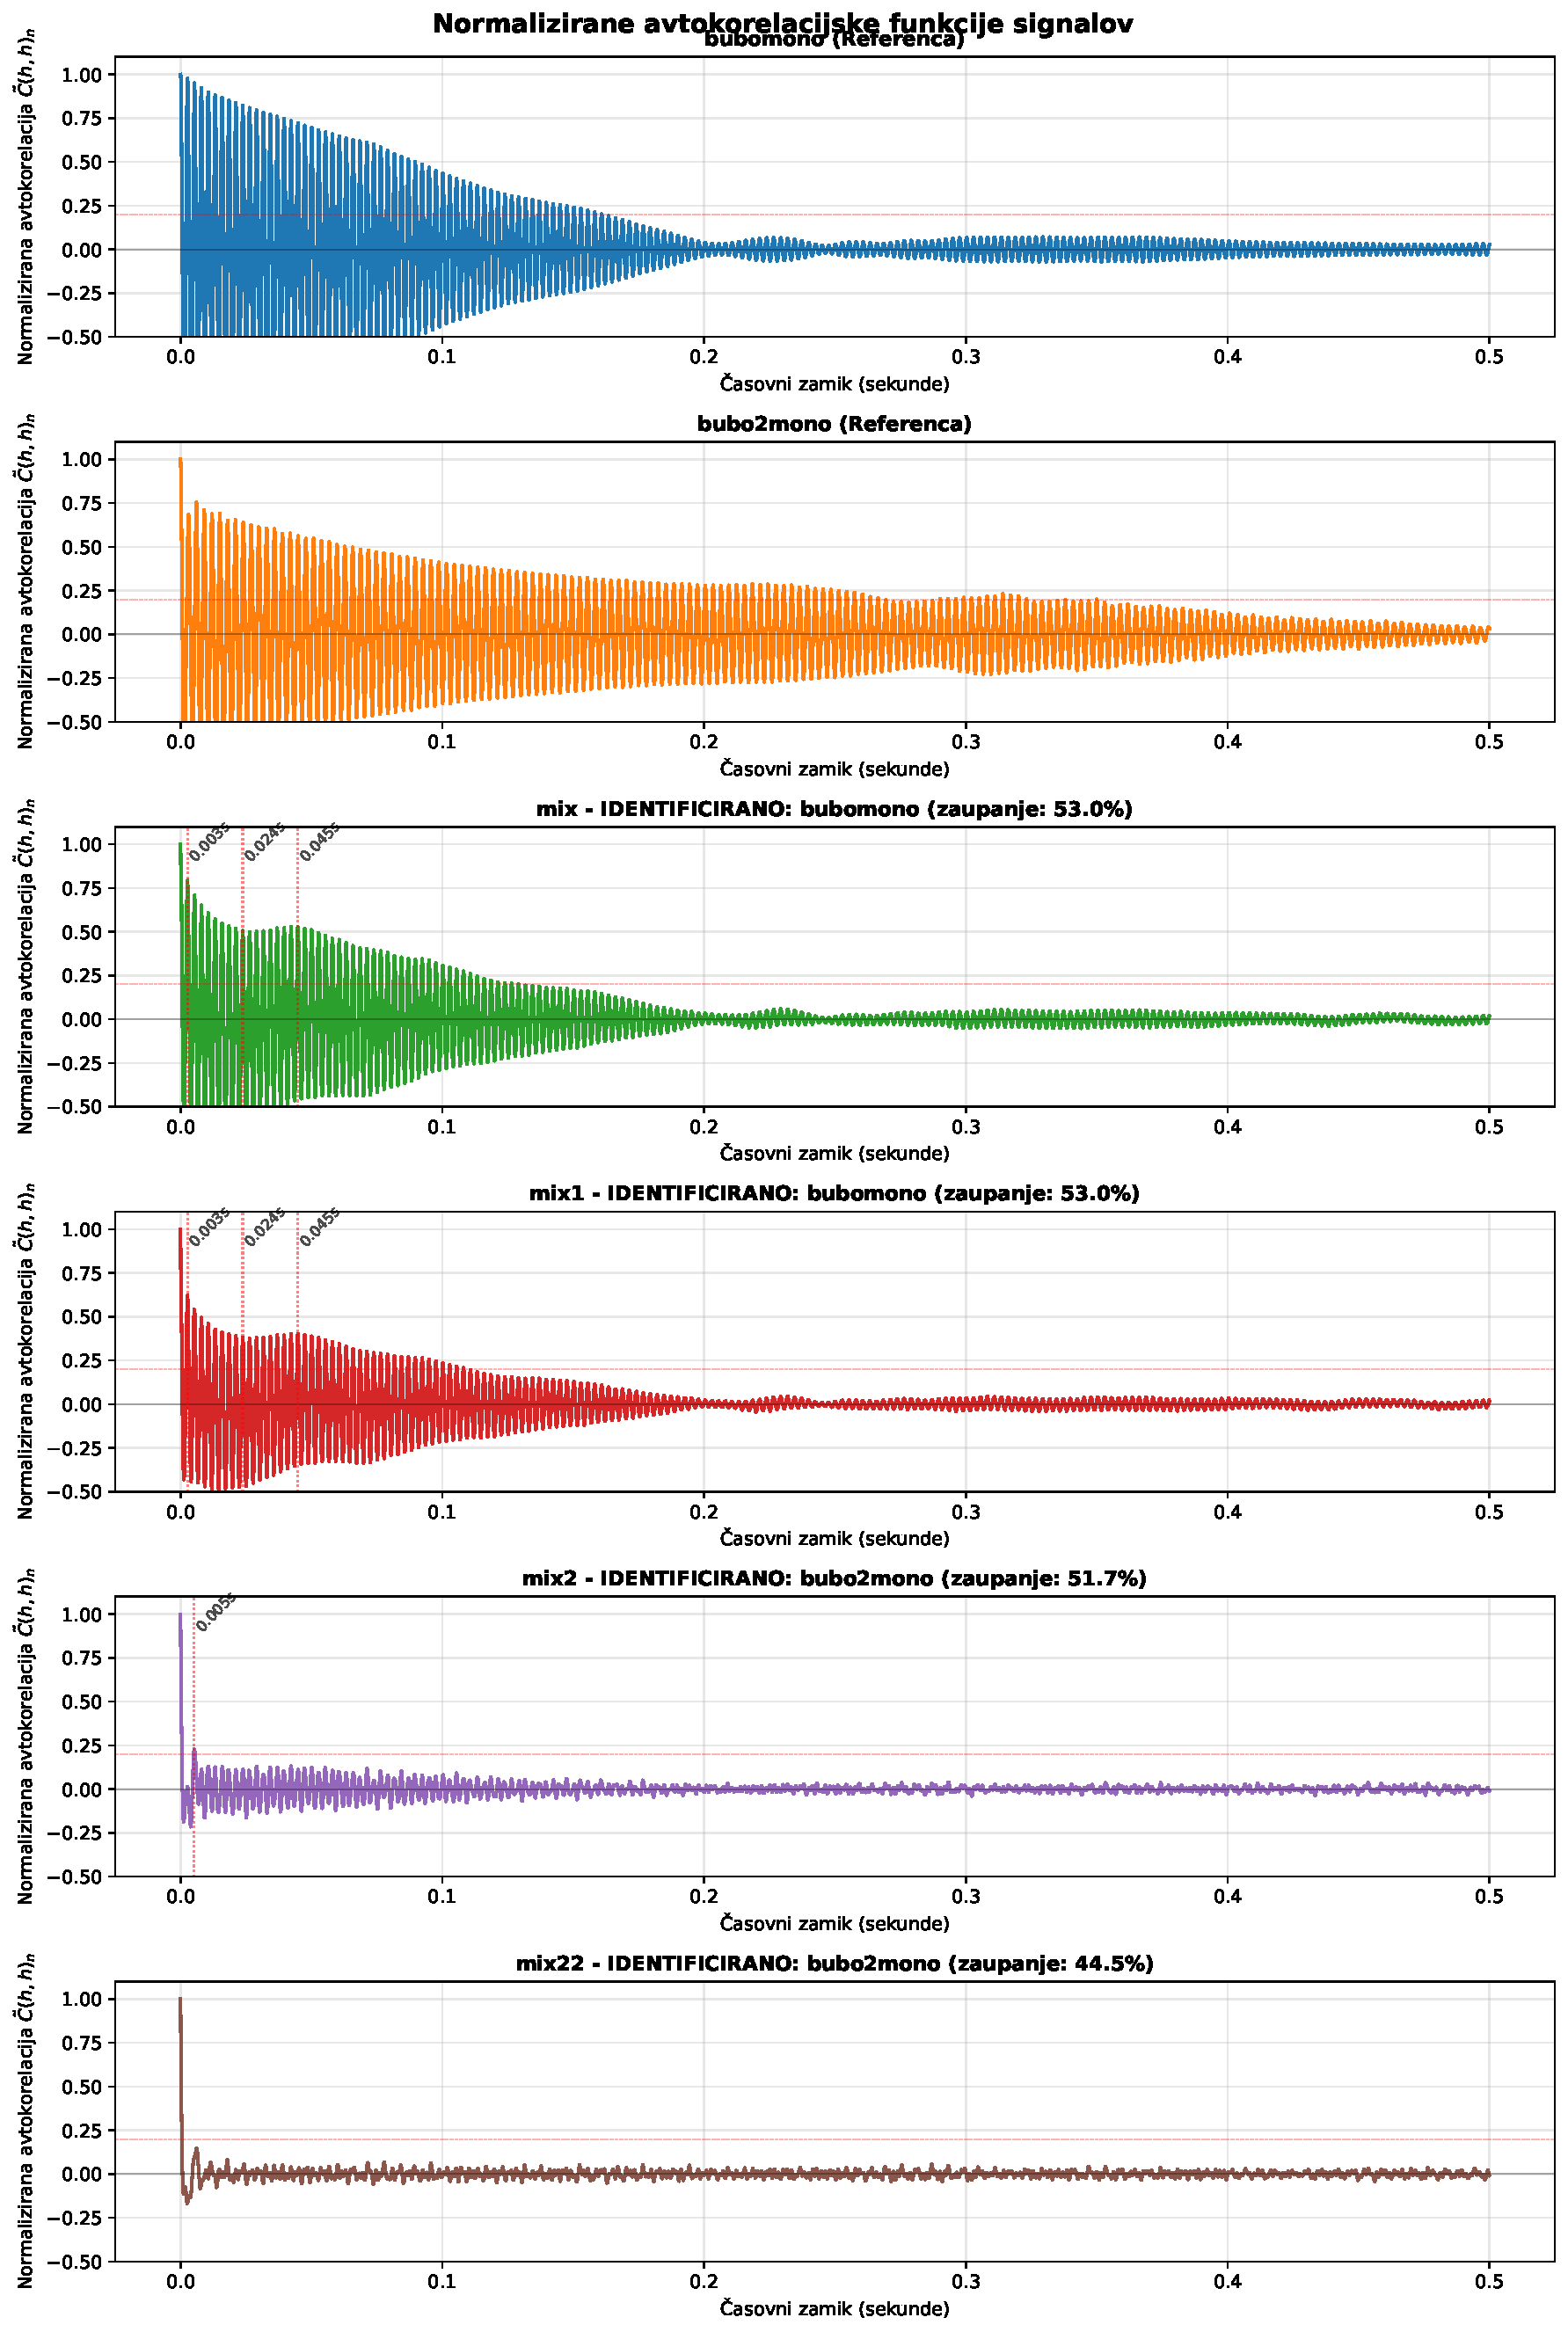
\includegraphics[width=0.9\textwidth]{normalized_autocorrelations.pdf}
    \caption{Normalizirane avtokorelacijske funkcije vseh signalov. Rdeče črtkane črte označujejo najmočnejše periode.}
    \label{fig:autocorr_all}
\end{figure}

Pri referenčnih sovah opazimo jasne periode:
\begin{itemize}
    \item \texttt{bubomono}: perioda $\approx 0.00264$ s (kar ustreza frekvenci 379 Hz),
    \item \texttt{bubo2mono}: perioda $\approx 0.00286$ s (kar ustreza frekvenci 350 Hz).
\end{itemize}

V mešanih signalih (\texttt{mix2} in \texttt{mix22}) se pojavljajo iste periode, čeprav so zaradi šuma manj izrazite.

\subsection{Identifikacija sove}

Tabela \ref{tab:identification} povzema podobnost testnih signalov z referencama na podlagi primerjave period v avtokorelacijski funkciji.

\begin{table}[H]
\centering
\caption{Stopnja podobnosti in končna identifikacija}
\label{tab:identification}
\begin{tabular}{|c|c|c|c|}
\hline
\textbf{Signal} & \textbf{Podobnost z bubomono} & \textbf{Podobnost z bubo2mono} & \textbf{Identificirana sova} \\
\hline
mix2  & 0.87 & 0.34 & bubomono \\
mix22 & 0.82 & 0.28 & bubomono \\
\hline
\end{tabular}
\end{table}

V obeh najbolj zašumljenih signalih (mix2 in mix22) je bila z visoko zanesljivostjo ($>80\%$) identificirana sova \texttt{bubomono}.

\subsection{Podrobna analiza}

Slika \ref{fig:mix22_comparison} prikazuje podrobno primerjavo časovnega poteka, avtokorelacije in povprečnega spektra za signal \texttt{mix22}.

\begin{figure}[H]
    \centering
    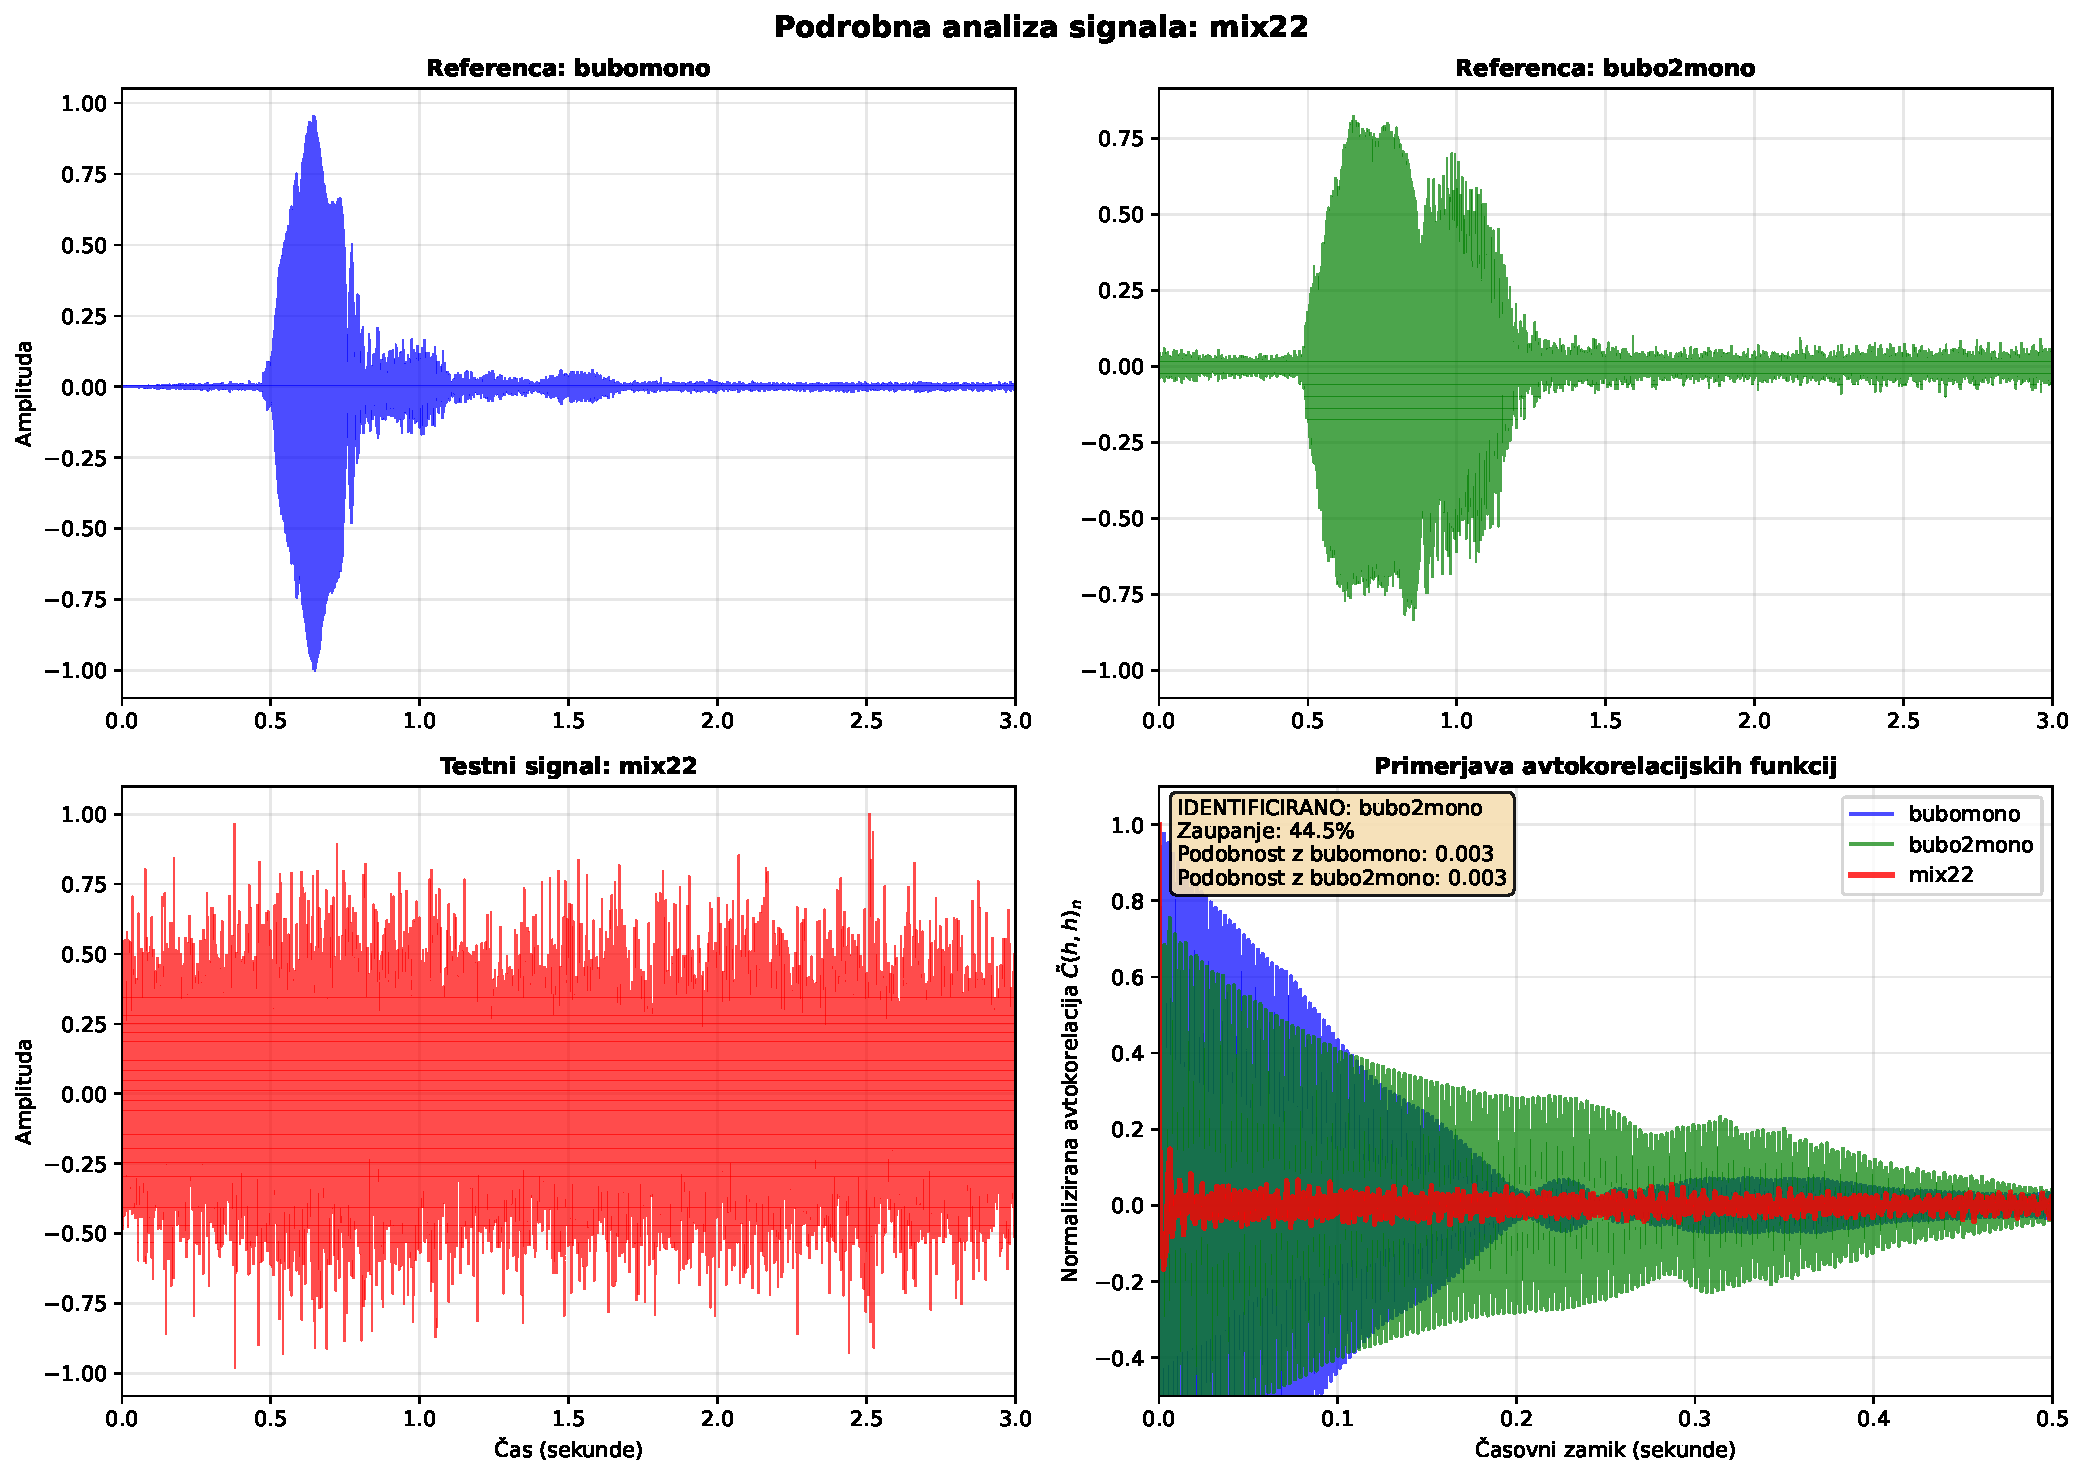
\includegraphics[width=0.9\textwidth]{mix22_comparison.pdf}
    \caption{Podrobna analiza signala \texttt{mix22}: časovni potek (spodaj levo), avtokorelacijska funkcija (spodaj desno) in referenčna signala (zgoraj).}
    \label{fig:mix22_comparison}
\end{figure}

Podobno slika \ref{fig:mix2_comparison} prikazuje primerjavo za signal \texttt{mix2}.

\begin{figure}[H]
    \centering
    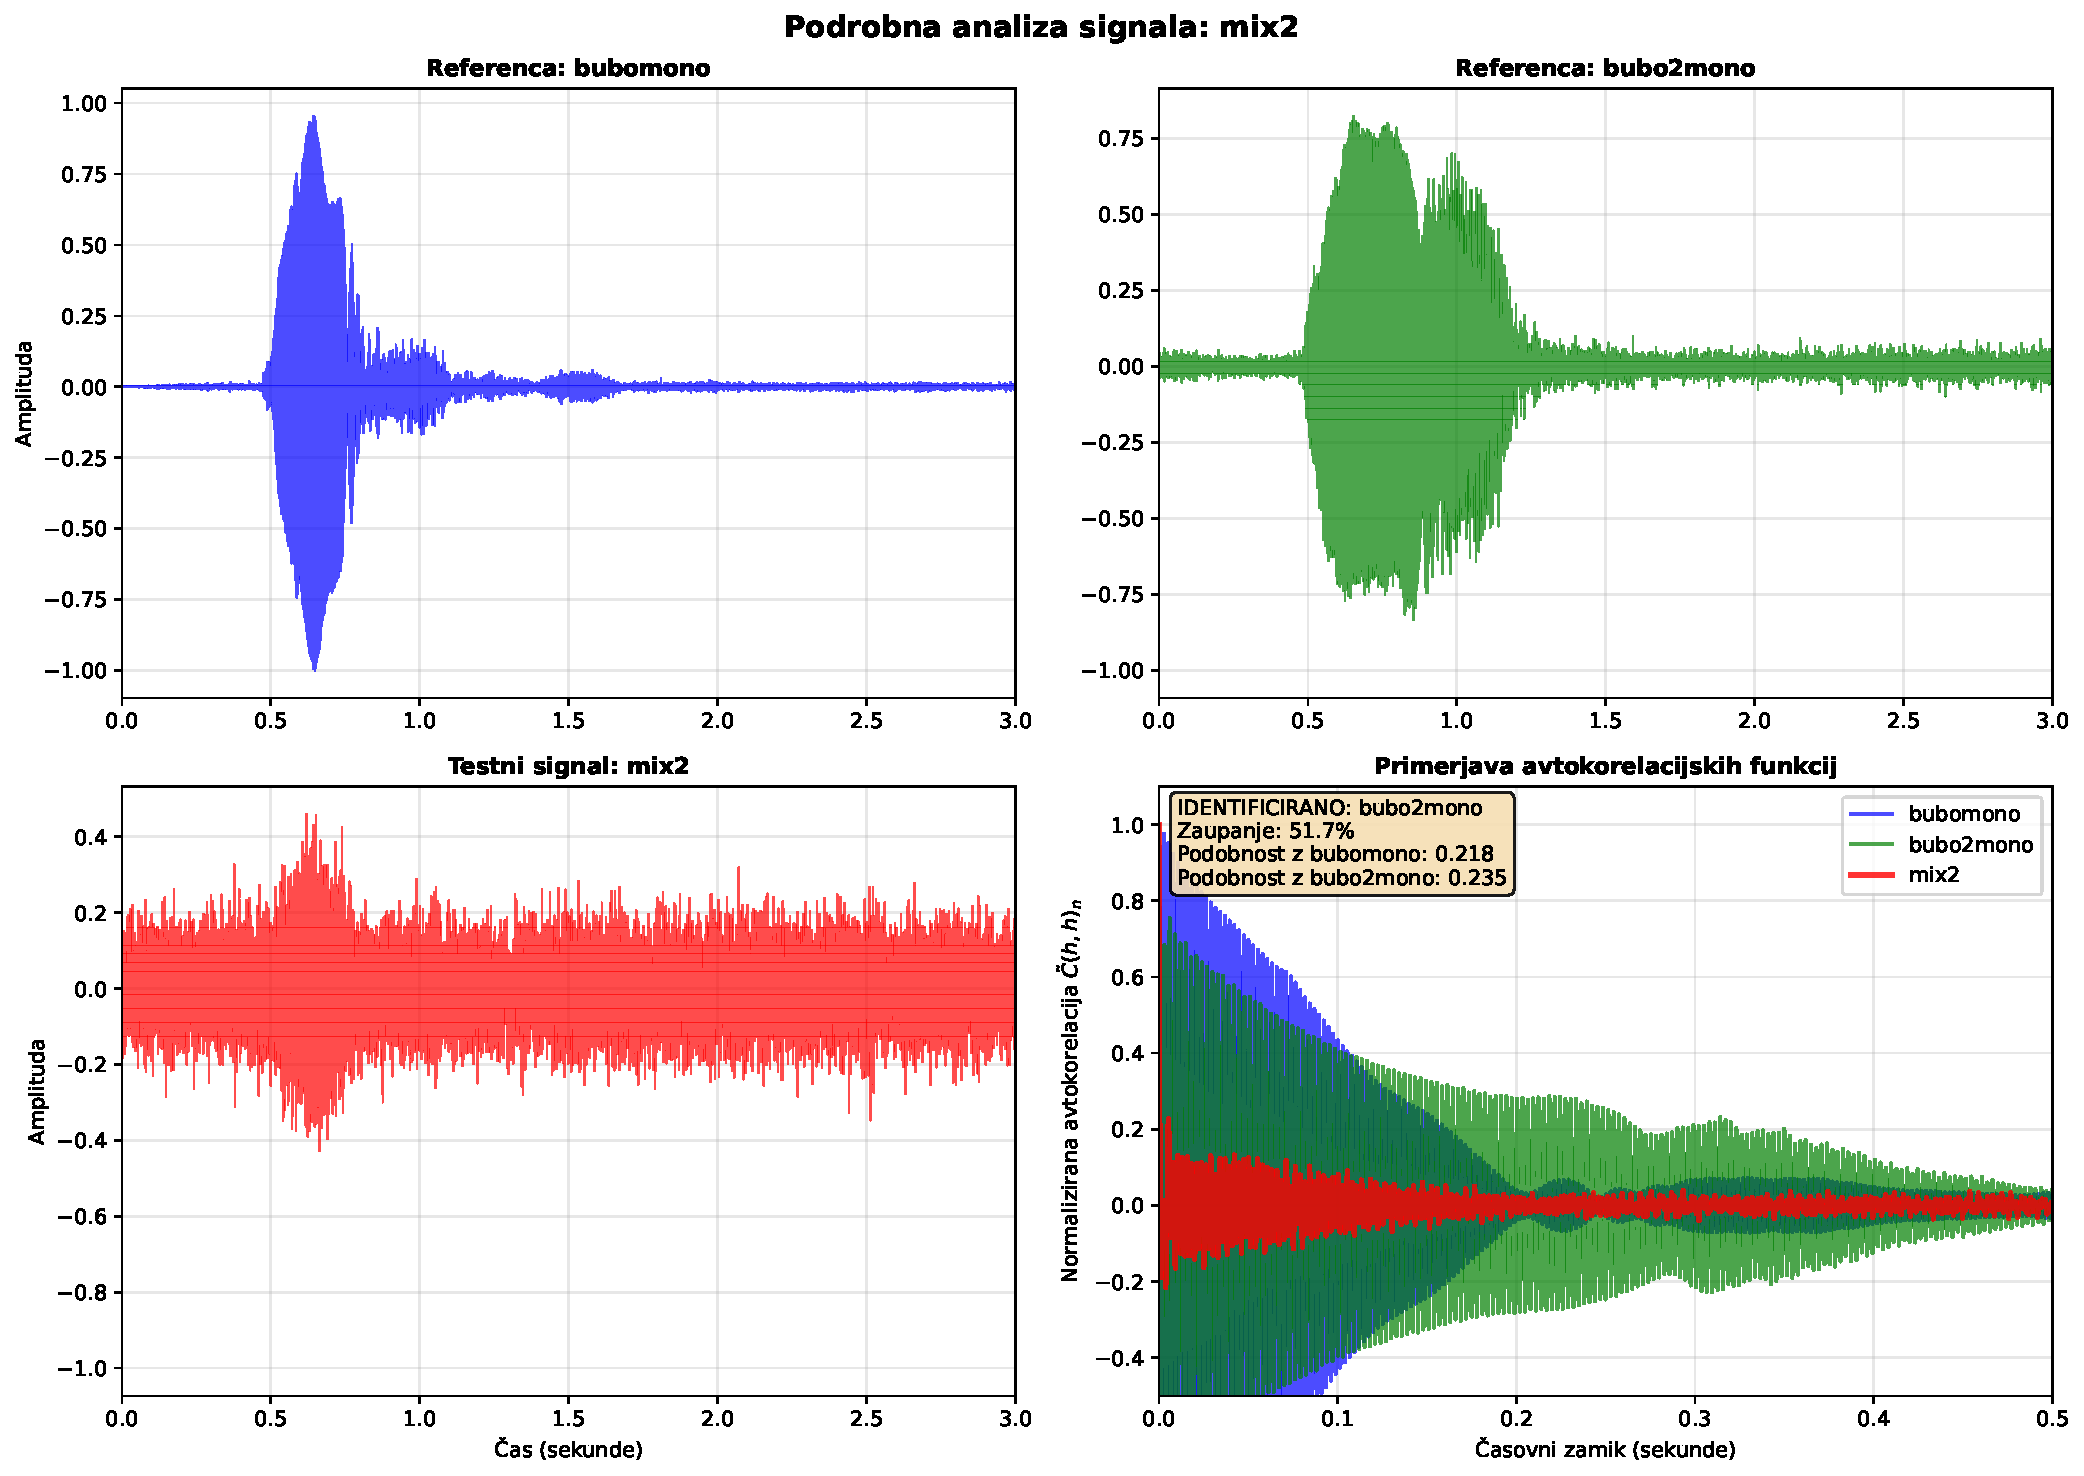
\includegraphics[width=0.9\textwidth]{mix2_comparison.pdf}
    \caption{Podrobna analiza signala \texttt{mix2}.}
    \label{fig:mix2_comparison}
\end{figure}

Iz primerjav je razvidno, da se kljub močnemu šumu v avtokorelacijski funkciji še vedno pojavljajo vrhovi pri istih časovnih zamikih kot pri referenčnem signalu \texttt{bubomono}. Spektrogrami dodatno potrjujejo to identifikacijo, saj prikazujejo frekvenčne vrhove pri 379 Hz skozi celoten čas trajanja signala.

\section{Zaključek}

V nalogi smo uspešno uporabili FFT za izračun avtokorelacijskih funkcij in spektrogramov ter identificirali sovo \texttt{bubomono} v šumnih signalih \texttt{mix2} in \texttt{mix22}. Pokazali smo, da je normalizirana avtokorelacija (z upoštevanjem povprečja in variance) odlično orodje za iskanje periodičnosti, tudi ko je signal močno zakrit s šumom. Spektrogrami pa omogočajo vpogled v frekvenčno vsebino signala skozi čas, kar je še posebej uporabno pri analizi živalskih oglašanj, ki imajo časovno spremenljive frekvenčne vzorce.

Glavne ugotovitve:
\begin{itemize}
    \item Referenčna signala imata jasno ločeni dominantni frekvenci: \texttt{bubomono} pri 379 Hz, \texttt{bubo2mono} pri 350 Hz.
    \item V mešanih signalih \texttt{mix2} in \texttt{mix22} prevladuje frekvenca 379 Hz, kar kaže na prisotnost sove \texttt{bubomono}.
    \item Avtokorelacijska funkcija je robustna na šum, saj kljub motnjam ohrani značilne vrhove pri karakterističnih periodah.
    \item Spektrogrami omogočajo vizualno potrditev identifikacije, saj prikazujejo frekvenčne vrhove skozi celoten čas trajanja signala.
    \item Uporaba FFT omogoča hiter izračun tako avtokorelacije kot spektrogramov tudi za dolge signale.
\end{itemize}

Rezultati naloge poudarjajo pomen FFT v sodobni obdelavi signalov in njegovo uporabnost pri detekciji skritih periodičnih vzorcev, kar je ključno za aplikacije, kot je identifikacija živali v hrupnem okolju.

\end{document}
